\documentclass[convert={density=300,size=1080x800,outext=.png}]{standalone}
\usepackage{xcolor}
\usepackage{graphics, graphicx}
\usepackage{tikz, tkz-graph}
\usepackage{pgf, pgfplots}
\usepackage{graphviz, tkz-berge}
\usepackage{graphics, graphicx}
\usepackage{pstricks, pst-node, pst-tree}

\usetikzlibrary{arrows, petri, topaths}
\usetikzlibrary{shapes}
\usetikzlibrary{arrows.meta}
\usetikzlibrary{positioning,automata}



\begin{document}
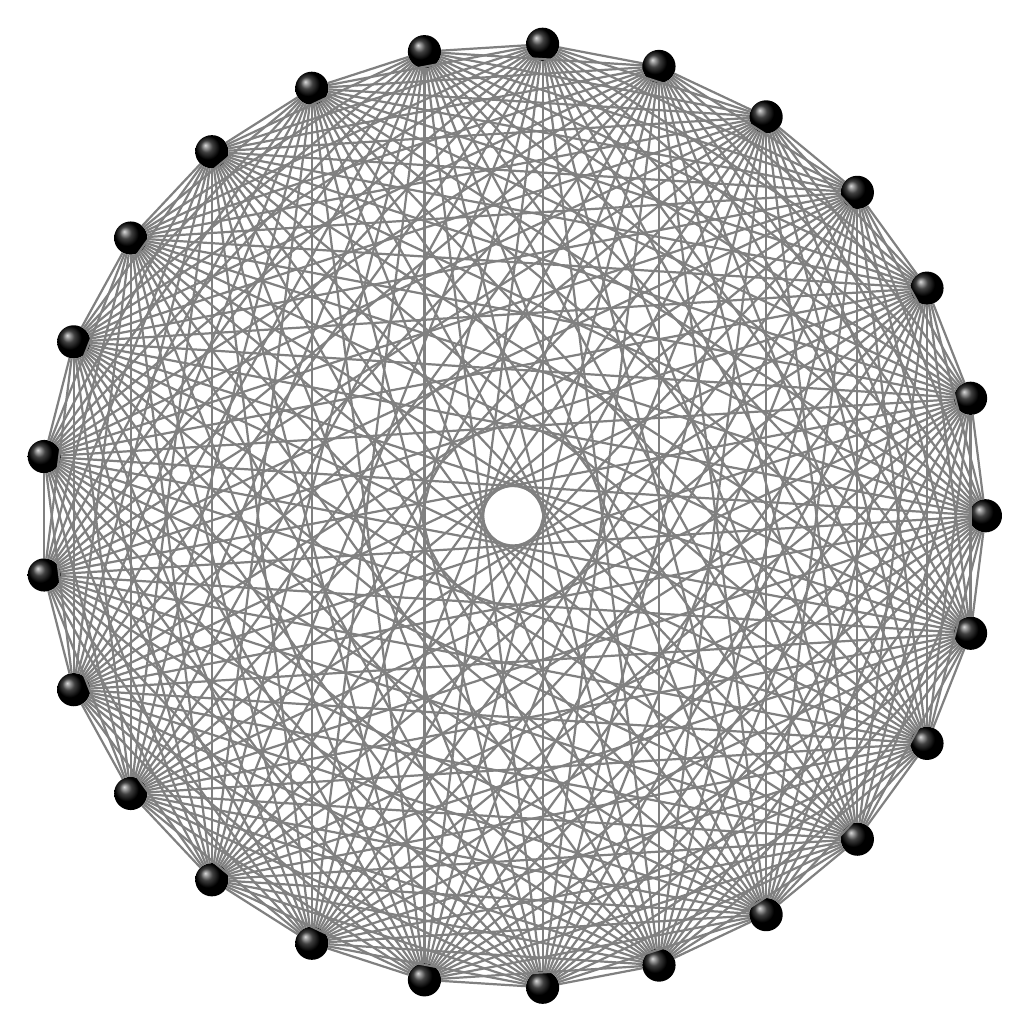
\begin{tikzpicture}[transform shape,line width=0.2pt]
 \SetVertexNoLabel
  \GraphInit[vstyle=Art]
  \SetGraphArtColor{black}{gray}
 %\grBalaban[form=3,RA=7,RB=6.5,RC=5.6,RD=5.6,RE=4.6]
 \grCirculant[RA=6]{25}{1,2,3,4,5,6,7,8,9,10,11,12}
%  \foreach \x in {1,...,16}{%
%    \pgfmathparse{(\x-1)*45+floor(\x/9)*22.5}
%    \node[draw,circle,inner sep=0.25cm] (N-\x) at (\pgfmathresult:5.4cm) [thick] {};
%  } 
%  \foreach \x [count=\xi from 1] in {2,...,16}{%
%    \foreach \y in {\x,...,16}{%
%        \path (N-\xi) edge[-] (N-\y);
% }
%}
\end{tikzpicture}
\end{document}